\documentclass[a4paper,12pt]{report}
\usepackage{times}
\usepackage{graphicx}
\usepackage[a4paper,
bindingoffset=0.2in,
left=1in,
right=.5in,
top=.7in,
bottom=.5in,
footskip=.25in]{geometry}
\usepackage{pdfpages}
\begin{document}
	\begin{center}
		\textbf{NETACODE -A SOFTWARE COMPANY VISITING REPORT}\\
		\begin{flushleft}
			The report is visiting a software company for \textbf{Course tittle:Information System Design with industrial attachment Sessional} Course and \textbf{Course Code:CSE 3210} in Computer Science and Engineering.\\
		\end{flushleft}
				by\\	
			Mst.Habiba Hena Sumi(200101070)\\Most.Jannat-Ul-Ferdoush(200101068)\\Md.Talath Un Nabi(200101076)\\Ferdous Tahsin(200101079)\\
			
			\begin{figure}[h]
				\centering
				\includegraphics[width=0.4\linewidth]{"BAUST_logo.png"}
				\label{fig:images-1}
			\end{figure}
		
		\vspace{1 cm}
			Submited To:\\
			Teacher name:Ananna Hoque Shathi\\
			Department of Computer Science and Engineering(CSE)\\
			Bangladesh Army University of Science and Technology(BAUST)\\
			
		\end{center}
	
	\begin{flushright}
		\vspace{4 cm}
		...............................................\\
		signature of the teacher
	\end{flushright}
\newpage
\tableofcontents
\listoffigures
\newpage

\chapter{Systems Concepts and the Information Systems Environment}
\section{Introduction}
 System analysis and design is a process that many companies use to evaluate particular business situations and develop ways to improve them through more optimal methods.\\
 
\begin{figure}[h]
	\centering
	
\includegraphics[width=0.9\linewidth]{1_1}
	\label{fig:11}
\end{figure}

NetaCode Inc is one of the upgrowing diversified IT solutions Provider Company Registered in as "NetaCode" at Bangladesh in 2018. Later in 2020 it's incorporated as "NetaCode Inc" at Delware, USA.
\section{NetaCode goal}
Netacode goal is simple and one that combines creativity with the latest research and development in the tech
world.they are a very customer-oriented company, putting our customers first and always focusing on
gaining and deserving the trust of every single one of their customers. So, they listen to their customers, stay
at the cutting edge of the latest trends in tech research, and constantly develop better web hosting
products and services which enable them to fulfill this vision better and better every day.
\\
\\
 
To provide trouble-free, customer-focused, reliable, and affordable web hosting services. they simply want
to continue to operate a profitable web hosting company that makes customers happy. Since the
beginning, they have backed they rock solid hosting solutions and top-notch infrastructure with the best
customer service and technical support. A common feeling about the technology field is it's all about
machines, yes, It does take machines but, Host Pair also knows it takes good people to run a well-oiled
machine. Yes, a successful business needs to be committed to client solutions, innovation, creativity, and
a warm, caring attitude to all of our customers' business needs. We don't just provide 24x7 support. they
really do listen and care.
\section {Characteristic of System}
\textbf{Organization}
Their organization has a branch in Dinajpur district. Netacode is a multinational software company. Main office in Dhaka in Bangladesh. Their organizations are certainly very beautiful. 4 storied building and their number of rooms is 7.\\

\textbf{Interaction}
It is defined by the manner in which the components operate with each other.For example, in an organization,purchasing department must interact with production department and payroll with personnel department.\\

\textbf{Interdependence}
Interdependence means how the components of a system depend on one another. Netacode has different branch in bangladesh,the branch  are interdependence each other . \\

\textbf{Integration}
Integration is concerned with how a system components are connected together. It means that the parts of the system work together within the system even if each part performs a unique function.Netacode each branch connect in every work with each other.\\

\textbf{Central Objective}
The objective of system must be central. It may be real or stated. It is not uncommon for an organization to state an objective and operate to achieve another.
\\
Netacode central objective is provide trouble-free, customer-focused, reliable, and affordable web hosting services.
\begin{figure}[h]
	\centering
	
\includegraphics[width=0.7\linewidth]{1}
	\caption{Task Interdependence in a Computer – Based Subsystem }
	\label{fig:1}
\end{figure}
\section{Elements of System}
\textbf{Outputs and Inputs}
\begin{itemize}
	\item 	The main aim of a Netacode is to produce an output which is useful for its user.
	\item 	Output is the outcome of processing.
\end{itemize}
\textbf{Processor(s)}
\begin{itemize}
	\item 	The processor is the element of Netacode that involves the actual transformation of input into output.
\end{itemize}
\textbf{control}
\begin{itemize}
	\item Netacode control the pattern of activities governing input, processing, and output.
\end{itemize}
\textbf{Feedback}
\begin{itemize}
	\item Feedback provides the control in a dynamic system.Netacode follow always clint feedback,future work doing follow the feedback .
	\item	Positive feedback is routine in nature that encourages the performance of the system.
	\item	Negative feedback is informational in nature that provides the controller with information for action.
\end{itemize}
\textbf{Environment}
\begin{itemize}
	\item	The environment is the “supersystem” within which an organization operates.
\end{itemize}
\textbf{Boundaries and Interface}
\begin{itemize}
	\item	A system should be defined by its boundaries. Boundaries are the limits that identify its components, processes, and interrelationship when it interfaces with another system.
	\item	Netacode  has boundaries that determine its sphere of influence and control.
\end{itemize}
\begin{figure}[h]
	\centering
	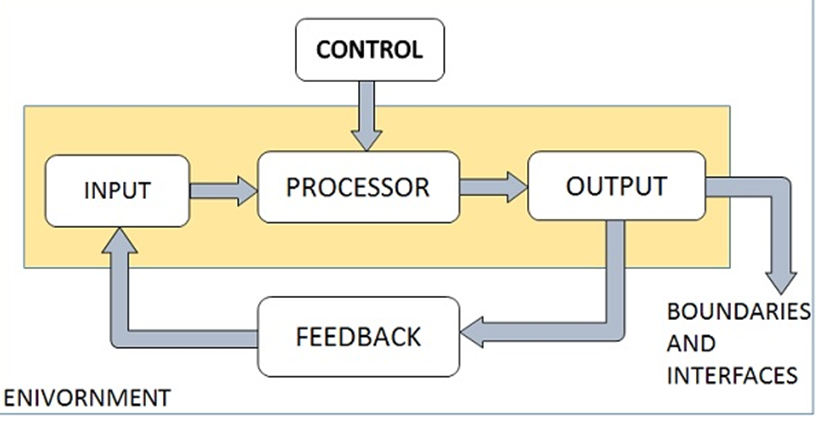
\includegraphics[width=0.7\linewidth]{2}
	\label{fig:2}
\end{figure}
\section{Types of Systems}
Netacode is a open and close system\\

\textbf{Open or Closed Systems}
\begin{itemize}
	\item	An open system must interact with its environment. It receives inputs from and delivers outputs to the outside of the system. For example, an information system which must adapt to the changing environmental conditions.
	\item	A closed system does not interact with its environment. It is isolated from environmental influences. A completely closed system is rare in reality.
\end{itemize}
\begin{figure}[h]
	\centering
	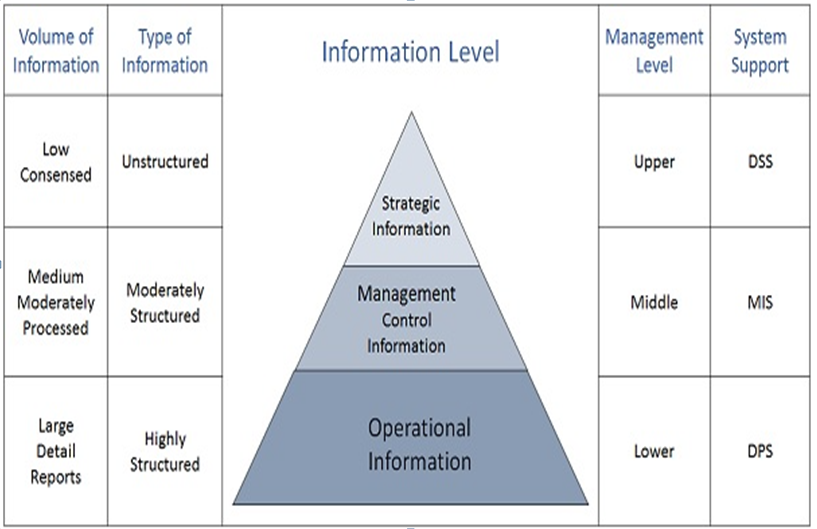
\includegraphics[width=0.7\linewidth]{3}
	\caption{Categories of information related to managerial levels and the decision managers make.}
	\label{fig:3}
\end{figure}
\textbf{Goals}\\
To provide trouble-free, customer-focused, reliable, and affordable web hosting services. WE simply want
to continue to operate a profitable web hosting company that makes customers happy. \\Since the
beginning, we have backed our rock solid hosting solutions and top-notch infrastructure with the best
customer service and technical support. A common feeling about the technology field is it's all about
machines, yes, It does take machines but, Host Pair also knows it takes good people to run a well-oiled
machine. Yes, a successful business needs to be committed to client solutions, innovation, creativity, and
a warm, caring attitude to all of our customers' business needs. We don't just provide 24x7 support. We
really do listen and care.
\section{Conclusion}

 we define the process of system analysis and design, outline the benefits of this process and list seven tools and techniques that may aid a organization in implementing its next system analysis and design process.
 The analyst plays many roles, sometimes balancing several at the same time. The three primary roles of the systems analyst are: consultant, supporting expert, and agent of change.The analyst is the key member of the Management Information System (MIS) and Decision Support System (DSS).





\newpage
\chapter{The System Development Life Cycle }
\section{Introduction}
The system development life cycle is a conceptual model used for project management that describes the stages involved in an information system development project,from an initial feasibility study through maintainence of the completed application. To understand system development,we need to recognize that a candidate system has a life cycle. The stages are shown below:
\begin{enumerate}
	\item   Recognititon of need / initial investigation
	\item	Feasibility Study
	\item	Analysis
	\item   Design
	\item	Implementation
	\item	Post-implementation and maintenance   
	\end{enumerate}
\begin{figure}[h]
	\centering
	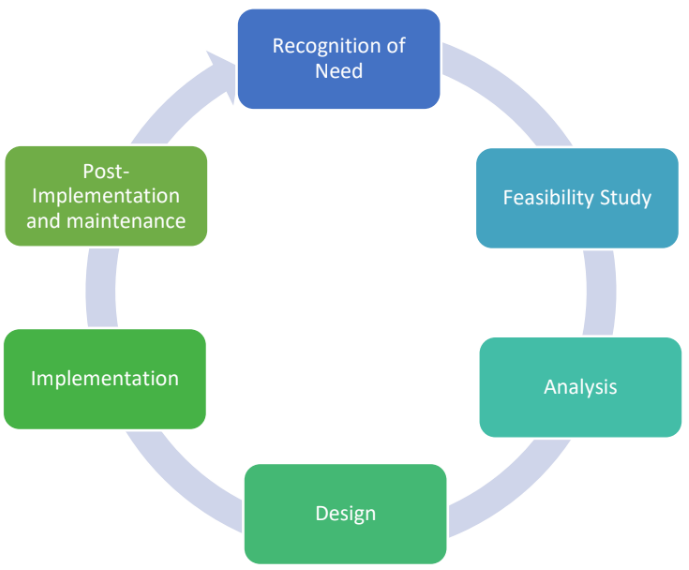
\includegraphics[width=0.7\linewidth]{2_1}
	\caption{System development life cycle}
	\label{fig:2_1}
\end{figure}
\section{Recognition of Need}
One must know what the problems are before it can be solved. The basis for a candidate system is recognition of a need for improving an information system or a procedure. For example, a supervisor wants to investigate the system flow in purchasing.When we have completed our visit at netacode ,we discuss the recognition needs of their clients and how they collect and process the requirements to complete their project  successfully. They told us they have arranged meetings with their clients many times to understand and collect the requirements. They provide them forms and other documents to understand what is the actual need of their clients.If the problem is serious enough , management may want to have an analyst look at it. Such assignment  implies a commitment. At this stage only a rough estimation of the development cost of the project may be reached.If the problem is serious enough , management may want to have an analyst look at it. Such assignment  implies a commitment. At this stage only a rough estimation of the development cost of the project may be reached.
\section{Feasibility Study}
Depending on the initial investigation the survey expanded to a more detailed feasibility study. It is the test of a system proposal according to its workability. It focuses on three major questions:
\begin{enumerate}
	\item 	What are the users demonstrable needs and how does a candidate system meet them?
	\item	What resources are available for a given candidate system? Is the problem worth solving?
	\item	What are likely impacts of the candidate system on the organization? How does it fit within the organization MIS plan?
	\end{enumerate}
Each of these questions must be answered carefully. They revolved around the investigation and evaluation of the problem,identification and description of the candidate system,specification of performance and the cost of each system and final selection of the best system.\\ \\
The proposal summarizes what is known and what is going to be done. It is consist of the following:
\begin{enumerate}
	\item \textbf{Statement of the problem :} A carefully worded statement of the problem led to analysis.
	
	\item \textbf{	Summary of the findings and recommendations :} A list of the major findings and recommendations of the study. It is the idea for the user who requires quick access to the results of the analysis of the system under study. Conclusions are started followed by a list of the recommendations and a justification for them.
	
	\item \textbf{ Details of the findings :} an outline of the methods are procedures undertaken by the existing system,followed by coverage of the objectives and procedures of the candidate system. Included are also discussions of output reports, file structures, and cost and benefits of the candidate system.
	
	\item \textbf{	Recommendation and conclusions :} Specific recommendations regarding the candidate system, including personnel assignments, costs, project schedules and target dates.
\end{enumerate}
\section{Analysis}
 It is the detailed study of the various operations performed by netacode  and their relationships within and outside of the system. A key question is : what must be done to solve the problem?\\ 
 
 When we visited the organization we discussed the analysis system. They first analys if they are able to complete it or not and then they discuss further processes that are steps they should take to make the project successful. Training, experience and common sense are required for collection of the information needed to do the analysis.
 \\ \\
 Once the analysis is completed, the analyst has a firm understanding what is to be done. The next step is to decide how the problem must be solved. Thus in system design, we move from the logical to physical aspects of the life cycle of a project.\\
 \section{Design}
 The most creative and challenging phase of a system life cycle of a project is system design. The term design describes a final system and the process by which it is developed. It refers to the technical specifications that will be applied in implementing the project. The question is here: How should the problem be solved?\\
 
\begin{figure}[h]
	\centering
	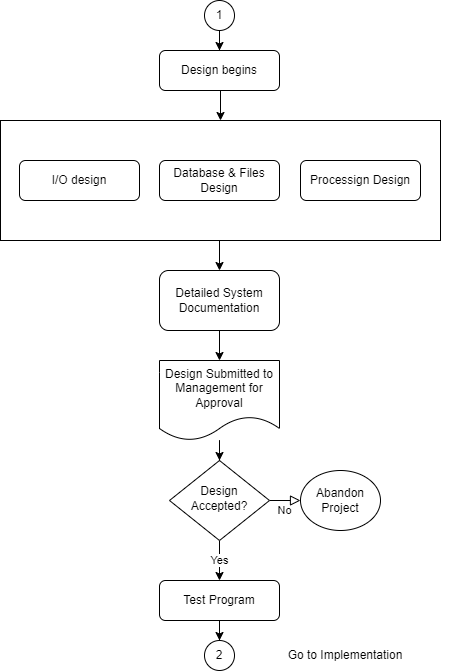
\includegraphics[width=0.7\linewidth]{2_2.png}
	\caption{design of a system}
	\label{fig:2_2}
\end{figure}
The first step is to determine how the output is to be produced and in what form. Samples of the output are also presented. Second, input data and master files  are designed to meet the requirements of the proposed output. Finally details related to justification of the project and an estimate of the impact of the candidate system on the user and the organization  are documented and evaluated by management as a step toward implementation.
\\ \\
In netacode they first create a virtual design of the project by adobe illustrator or figma.then they present it to their clients to justify if it has been according to their requirements or not.\\
In some firms, separate groups of programmers do the programming , whereas other firms employ analyst programmers who do analysis.
\section{Implementation}
The implementation sector is less creative than system design. It is primarily concerned with user training, site preparation and file conversion. Depending on the nature of the system, extensive user training may be required. Conversion usually takes place at about the same time the user is being trained or later.\\

In netacode they told us they used  react js as frontend development and node js for backend development. They also use nuxt js and next js for development. They used php but now they have shifted to javascript. \\

Once the program becomes available,test data is read into the computer and  processed against the file(s) provided for testing. If successful, the program(s) is then run with live data. Otherwise  a diagnostic procedure is used to locate and correct errors in the program. In most conversions a parallel run is conducted where the new system runs simultaneously with the old system. 
\section{Post termination and Maintenance }
After the installation phase is completed and the user stuff is adjusted to the changes created by the candidate system, evaluation and  maintenance begin. Like any system, there is an aging process that requires periodic maintenance of hardware and software. If the new information is inconsistent with the design specifications, the changes have to be made. The importance of maintenance is to continue to bring the new system to standards.\\ 

The policy of Netacode is to serve their clients with the project they have created according to the requirements. but they don't share the source code of any project and if their updates are available, they do it take charges. This is their strategy of post implementation and maintenance of any project.
\section{Conclusion}
In this chapter, discuss about Netacode (a system) life cycle and how it handle projects problem and it's solving methods.







\chapter{The Role of the System Analyst}
\section{Introduction}
Systems analysts analyse how well software, hardware and the wider IT system fit the business needs of their employer or of a client. They write requirements for new systems and may also help implement them and monitor their effectiveness. Typical responsibilities of the job include: examining current systems.
\paragraph{System Analysis} 
A person who conducts a methodical study and evaluation of an activity such as a business to identify its desired objective in order to determine procedurs by which these objectives can be gained.
\section{System Analyst}
The systems analyst plays a key role in information systems development projects. The systems analyst works closely with all project team members so that the team develops the right system in an effective way. Systems analysts must understand how to apply technology to solve business problems. In addition, systems analysts may serve as change agents who identify the organizational improvements needed, design systems to implement those changes, and train and motivate others to use the systems.\\
\textbf{Netacode interpersonal skills relevant to systems work include the following: }\\
\textbf{Communication:}having the ability to articulate and speak the language of the user, a "flare" for mediation, and a knack for working with virtually all managerial levels in the organization.  \\
\textbf{Understanding}identifying problems and assessing their ramifications, having a grasp of company goals and objectives, and showing sensitivity to the impact of the system on people at work.
\subsection{Technical skills include}
\textbf{Creativity}helping users model ideas into concrete plans and develop ing candidate systems to match user requirements.\\ \\
\textbf{Problem solving}reducing problems to their elemental levels for analy sis, developing alternative solutions to a given problem, and delineating the pros and cons of candidate systems\\ \\
\textbf{Project management}scheduling, performing well under time con straints, coordinating teain efforts, and managing costs and expendi **\\ \\
\underline{\textbf{NetacodeInterpersonal and Technical skill necessary in system Development :}}

\begin{figure}[h]
	\centering
	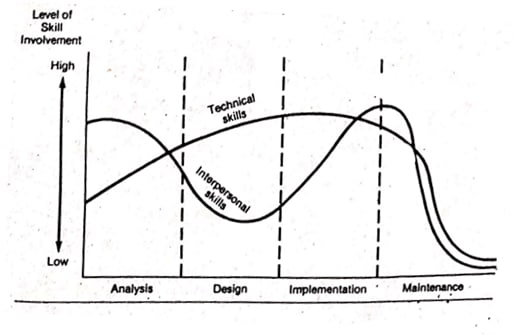
\includegraphics[width=0.9\linewidth]{3_1}
	\caption{Interpersonal and Technical Skills}
	\label{fig:31}
\end{figure}

\section{The attributes are}
\textbf{Authority-}the confidence to "tell" people what to do. Much of this quality shows in project management and team work to meet deadlines. Communication skills-ability to articulate and focus on a problem area for logical solution.\\
\textbf{Creativity-}trying one's own ideas, developing candidate systems using unique tools or methods.\\
\textbf{Hesponsibility-}making decisions on one's own and accepting the conequences of these decisions.\\
\textbf{Varied skills-}doing different projects and handling change.
\section{Conclusion}
A system analyst role to develop a project successfully,achieve the objectives.A system analyst need  technical and Interpersonal skill communication and interface with the user. Technical skills include creativity, problem solving, and managing the overall project.







\chapter{Systems Planning and the Initial Investigation}
\section{Bases for planning in system analysis}
It is a systematic approach, which uses graphical tools that analyze and refine the objectives of an existing system and develop a new system specification which can be easily understandable by user. It has following attributes: It is graphic which specifies the presentation of application.
\section{Strategic MIS Planning}
Planning for information system development must be done within the framework of the Netacodeoverall MIS plan. The time horizon dimension specifics whether it is short. which is tantamount to the MIS yearly plan medium term , or long range. 

 The first task in strategic planning is to set the MIS objectives and the results expected. 
 
 The next step is to devise short-range plans that spell out the day-to-day activities of the system. They are programmed plans requiring a year's commitment. For example, Netacode is operating expense budget, the human resource budget of each computer application, and timetables for implementing a new system are all short-range plans designed to implement the organization's master plan by computerizing the labor-intensive areas of the business.
\section{Strategies for Determining Information Requirements}
There are three key strategies or general approaches for eliciting information regarding the user's requirements:
\begin{enumerate}
	\item asking, \item Getting information from the existing information system, and \item Prototyping 
\end{enumerate}
\textbf{Asking} \\This strategy obtains information from users by simply asking them about the requirements. It assumes a stable system where users are well informed and can overcome biases in defining their problem.There are three key asking methods:
\begin{enumerate}
	\item Questions may be open-ended or closed. An open-ended question allows the respondent to formulate a response.for example, We ask some question about project development model and user handeling process etc to Netacode.
	\item Brainstorming is a technique used for generating new ideas and obtaining general information requirements.for example,We ask Netacode how they solve problem to buid a project.
	\item Group consensus asks participants for their expectations regarding specific variables a Delphi inquiry. for example,  Netacode worker  fills out a questionnaire The results are  summarized and given to worker along with a follow up questionnaire. Worker are invited to change their responses. The results are again summarized and feedback to the Netacode worker. This debate by questionnaire continues until participants responses have converged enough.
	
\begin{figure}[h]
	\centering
	\includegraphics[width=0.8\linewidth]{"amader pic"}
	\caption{Netacode jobholders and ours picture moment of getting information.}
	\label{fig:amader-pic}
\end{figure}
\end{enumerate}
\textbf{Getting information from the existing informaton system}
\\Netacode have 4 room and 20 worker .In this branch 18 is developer and programer.1 person is branch CEO,1 person is software architect.
\section{Conclusion}
	In this chapter, discuss about Netacode (a system) MIS planing and how we getting information from Netacode.
	




\chapter{Information Gathering}
\section{Introduction}
Information is stimuli that has meaning in some context for its receiver. When information is entered into and stored in a computer, it is generally referred to as data. After processing -- such as formatting and printing -- output data can again be perceived as information. When information is compiled or used to better understand something or to do something, it becomes knowledge.
\section{How Netacode collects information from clients}
\begin{figure}[h]
	\centering
	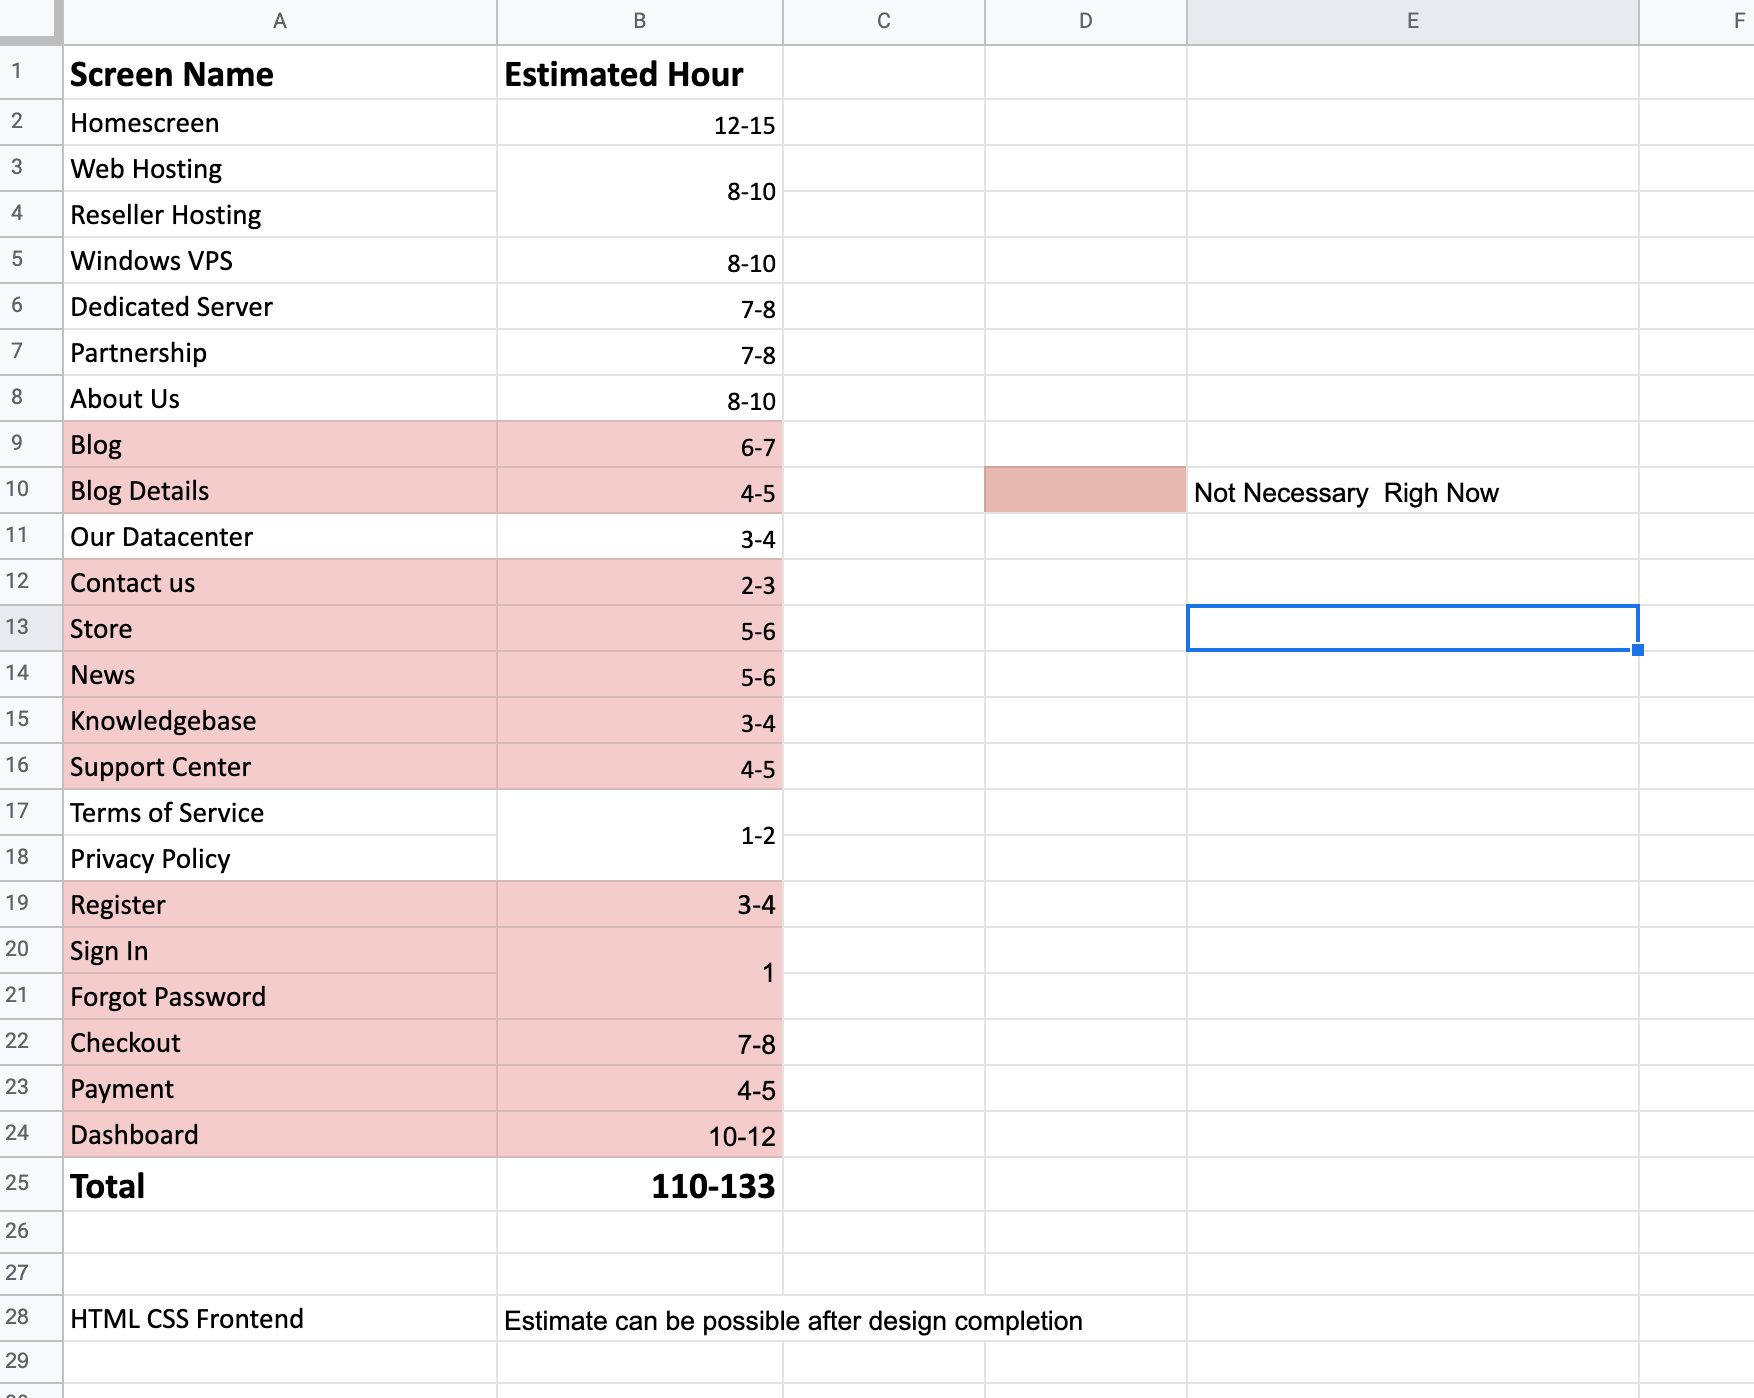
\includegraphics[width=0.7\linewidth]{5_1}
	\caption{Information Collection}
	\label{fig:51}
\end{figure}
Netacode uses various data collection tools to collect necessary information from clients. Then, they make project timeline according to the client's requirements. 
\section{Information about the firm}
The following Organization Chart for Netacode is displayed below.
\newpage
\begin{figure}[h]
	\centering
	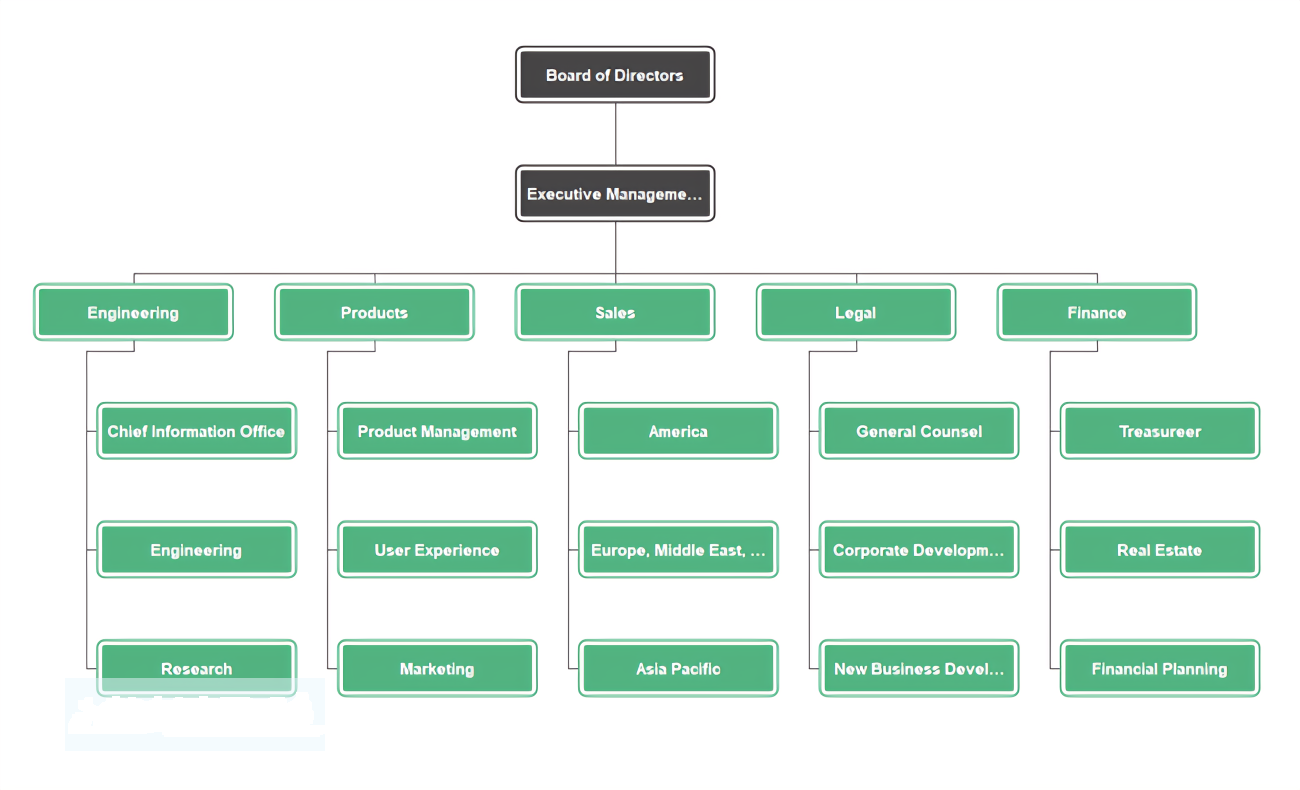
\includegraphics[width=0.9\linewidth]{5_2}
	\caption{Organization Chart of Netacode}
	\label{fig:52}
\end{figure}

\section{Information Gathering Method – Questionaries}
Since information must be acquired accurately, methodically, under the right conditions, and
with minimum interruption to user personnel there is some tools which have been used to gather
information. Though there are various kinds of information gathering tools we use:\\
\begin{enumerate}
	\item  Review of literature, procedures and forms.
	\item  On-site observation
	\item  Interviews
	\item Questionnaires
\end{enumerate}
In order to learn more about Netacode, we used a questionnaire form.
	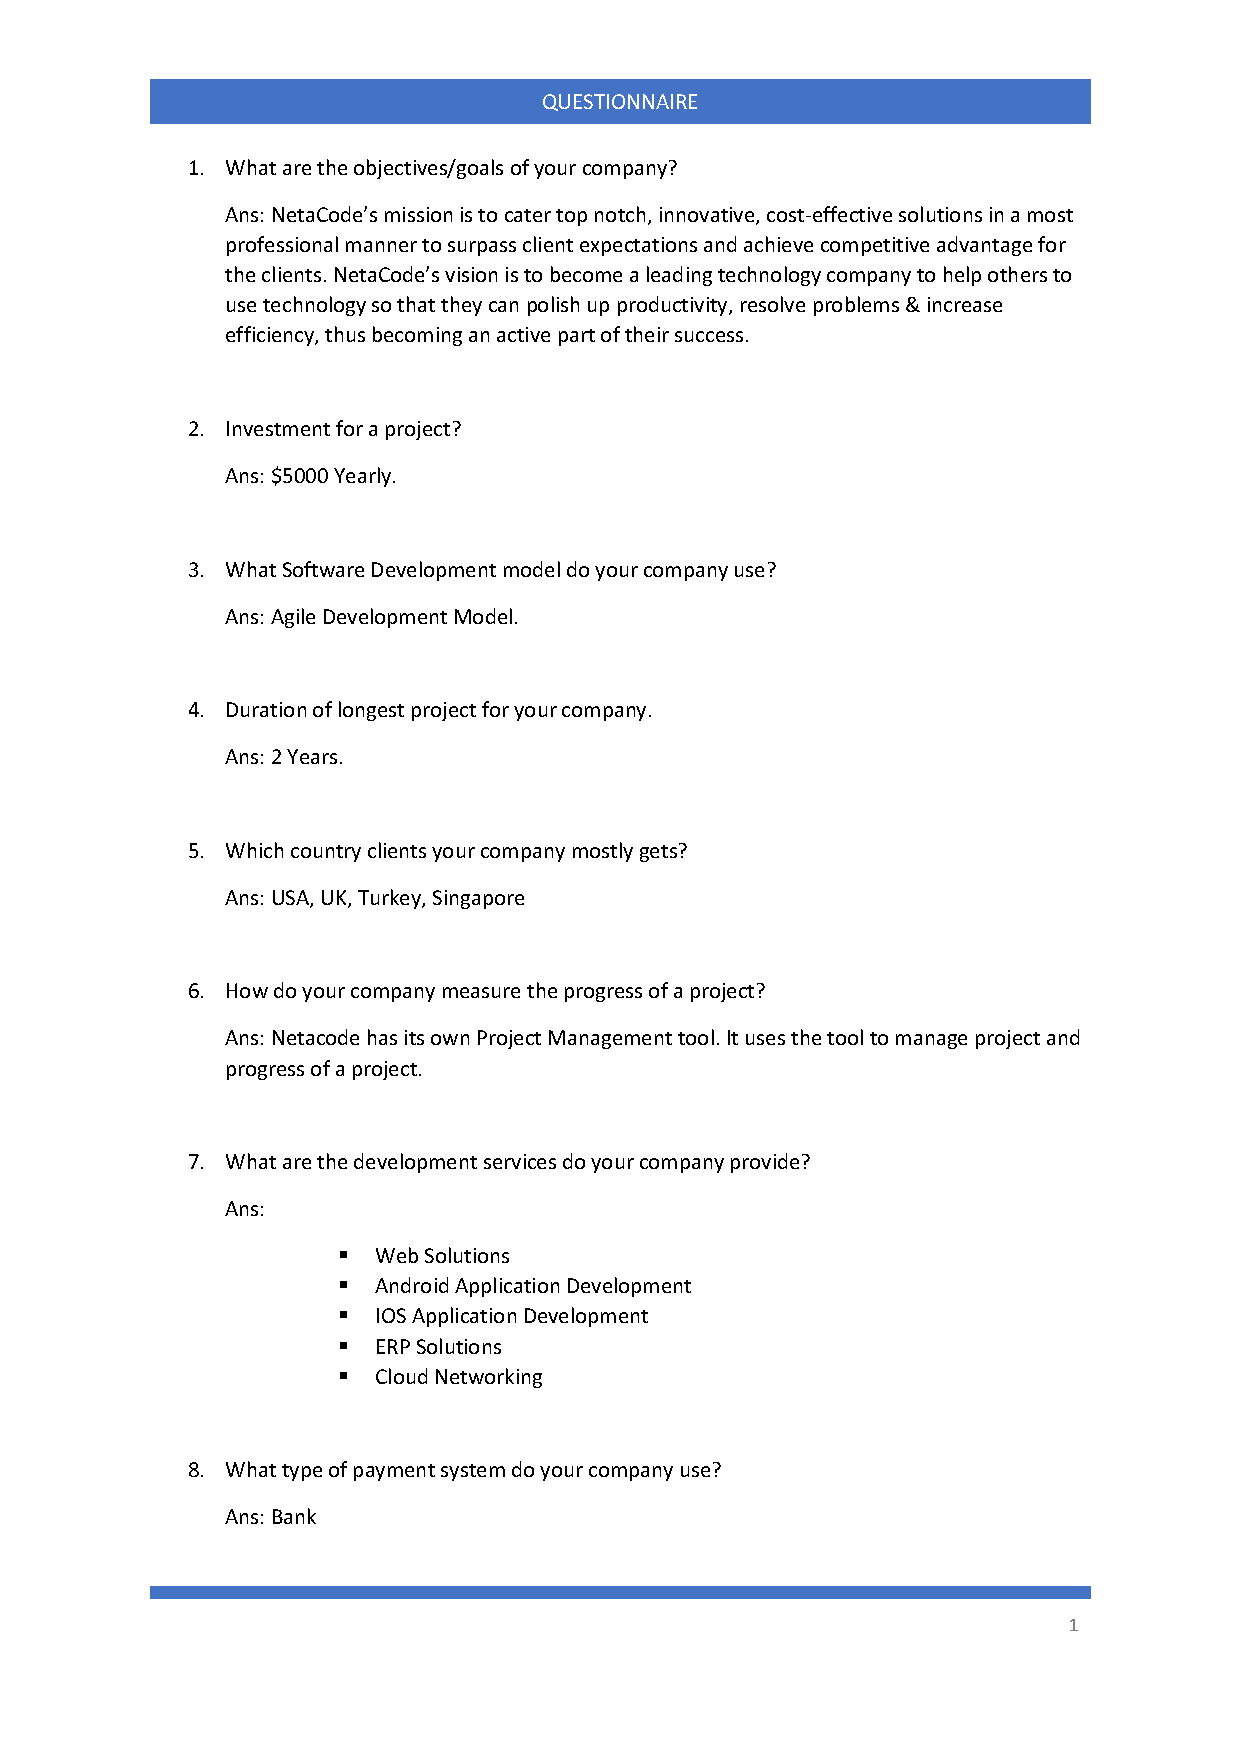
\includepdf[pages={1,2,3}] {5_questions.pdf}
\section{Conclusion}
This chapter taught us about numerous techniques for acquiring information as well as the Netacode company's organizational structure, which we visited. We also learned about the methods used by Netacode to gather client information.











\chapter{The Tools of Structured Analaysis}
\section{Structured Analaysis}
Structured Analaysis is a development method that allows the analyst to understand the system and its activities in a logical way.
It has following attributes 
\begin{itemize}
		\item	It is graphic which specifies the presentation of application. 
		\item	It divides the processes so that it gives a clear picture of system flow.  
		\item	It is logical rather than physical i.e., the elements of system do not depend on vendor or hardware.  
		\item	It is an approach that works from high-level overviews to lower-level details.
\end{itemize}
\section{Structured Analysis Tools}
During Structured Analysis, various tools and techniques are used for system development. They are \\
\begin{itemize}
	\item   Data Flow Diagrams
	\item	Data Dictionary
	\item	Decision Trees
	\item	Decision Tables
	\item	Structured English
	\item	Pseudocode
\end{itemize}
\begin{figure}[h]
	\centering
	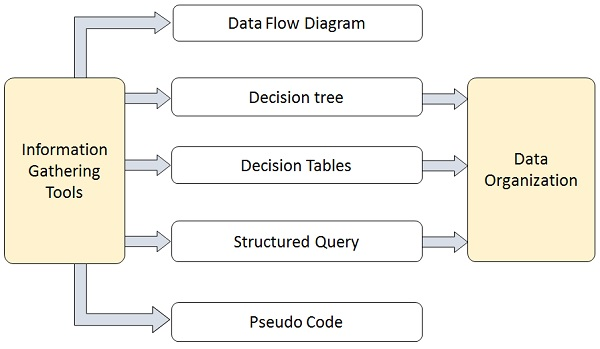
\includegraphics[width=0.7\linewidth]{6_fig1}
	\caption{Information Gathering Tools}
	\label{fig:6fig1}
\end{figure}
\section{Information Gathering Tools}
It is a technique developed by Larry Constantine to express the requirements of system in a graphical form.
\begin{itemize}
	\item 	It shows the flow of data between various functions of system and specifies how the current system is implemented.
	\item 	It is an initial stage of design phase that functionally divides the requirement specifications down to the lowest level of detail.
	\item 	Its graphical nature makes it a good communication tool between user and analyst or analyst and system designer.
	\item 	It gives an overview of what data a system processes, what transformations are performed, what data are stored, what results are produced and where they flow.
	
\end{itemize}
Standard symbols for DFDs are derived from the electric circuit diagram analysis and are shown in fig6.2:
\begin{figure}[h]
	\centering
	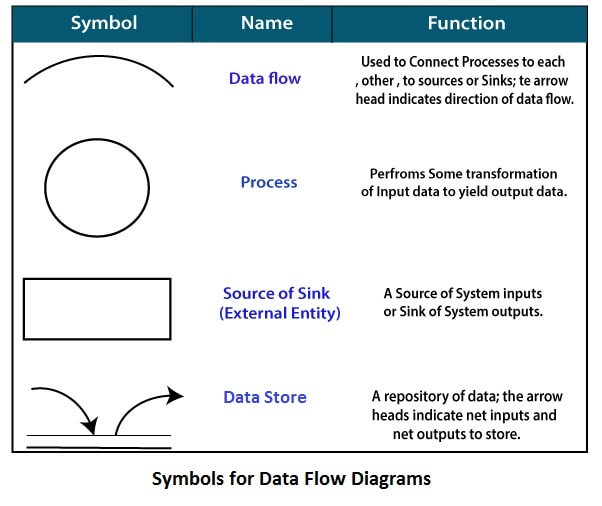
\includegraphics[width=0.7\linewidth]{6_fig2}
	\caption{Data Flow Diagram Symbols}
	\label{fig:6fig2}
\end{figure}
\newpage
Here is a Data Flow Diagram that Netacode provided, illustrates the data flow between their website, web server and database.

\begin{figure}[h]
	\centering
	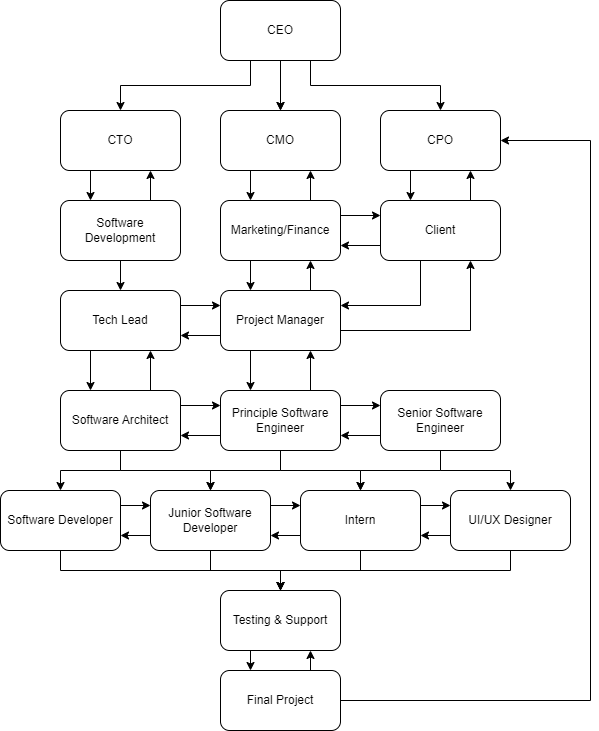
\includegraphics[width=0.9\linewidth]{dfd_company}
	\caption{Data Flow Diagram of Netacode}
	\label{fig:dfd_company}
\end{figure}
\newpage
Here Netacode billing system flow diagram

\begin{figure}[h]
	\centering
	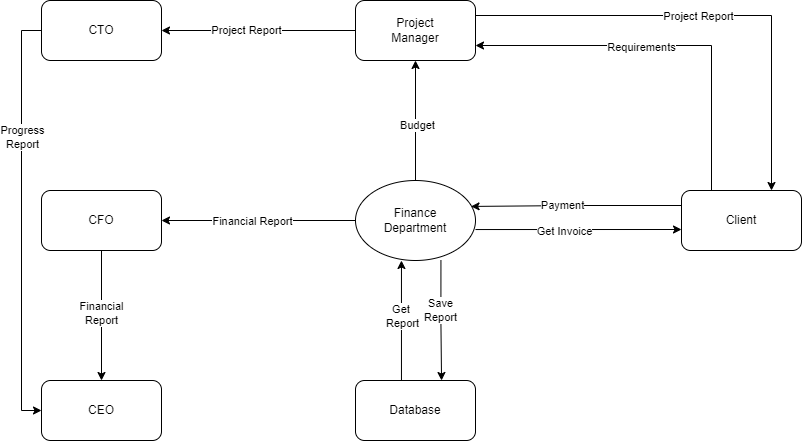
\includegraphics[width=0.9\linewidth]{dfd_company2}
	\caption{Netacode billing system}
	\label{fig:dfdcompany2}
\end{figure}
\section{Conclusion}
This chapter taught us about how make a system data flow diagram.Netacode data flow diagram and biling system also given in the chapter.











\chapter{Feasibility Study}
\section{Introduction}
A feasibility study in software engineering is a rigorous evaluation of the profitability and viability of a software development initiative.For a  company with 10-year expertise, ScienceSoft helps businesses understand whether a new software project is worth their time and money.
\\Feasibility Study Process : \\
\begin{enumerate}
	\item	Information assessment
	\item Information collection
	\item Report writing
	\item General information
\end{enumerate}
The next step is to determine exactly candidade system needed.\\
\section{Need of Feasibility Study in The Company} 
Feasibility study is so important stage of Software Project Management Process as after completion of feasibility study it gives a conclusion of whether to go ahead with proposed project as it is practically feasible or to stop proposed project here as it is not right/feasible to develop or to think/analyze about proposed project again
\section{System Performance}
Performance is an indicator of how well a software system or component meets its requirements for timeliness. Timeliness is measured in terms of response time or throughput. The response time is the time required to respond to a request. It may be the time required for a single transaction, or the end-to-end time for a user task. For example,Netacode determine performance clint response to want make project by them and clint feedback about existing project.\newpage
\begin{figure}[h]
	\centering
	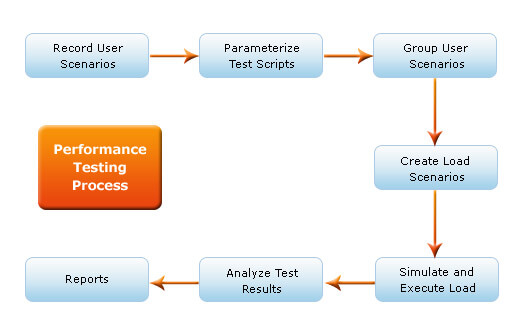
\includegraphics[width=0.8\linewidth]{Performance-Testing-Process}
	\caption{System performance diadram}
	\label{fig:performance-testing-process}
\end{figure}
\section{Identification of Specific System Objective}
In netacode a build a project and not sell the project ,they rent every project for a certain time(1 year).They must follow the below technique to build a project successfully.
\begin{enumerate}
	\item Live Chat and Ticket Review system
	\item Asking them over the phone.
	\item Listening to them carefully.
	\item Web Reviews
	\item Comment Sections
	\item Keyword Research
\end{enumerate}
\section{Feasibility Consideration}
\subsection{Economic Feasibility}
NetaCode give customer a 30-day money back guarantee, incase clients are not happy with our service.their hosting packages are scalable- clients can upgrade/downgrade as per clint needs.
No hidden prices.
\subsection{Technical Feasibility}
Since they rent the software, they handle all the technical issues themselves, they keep the software on their own multiple servers.
\subsection{Behaviour Feasibility}
Computer and device are not khow about what they do.what we want we can do everything with clint.So every project must know the behaviour with clint.
\subparagraph{}
For successfully run a project NetaCode flow 5 steps with in 8 step for Feasibility Analysis.
\begin{itemize}
	\item form a project team and appoint a project leader
	\item prepare system flowchart.
	\item select a template which  already build by them
	\item prepare and report final project directive to management
	\item select best candidate system
	\begin{figure}[h]
		\centering
		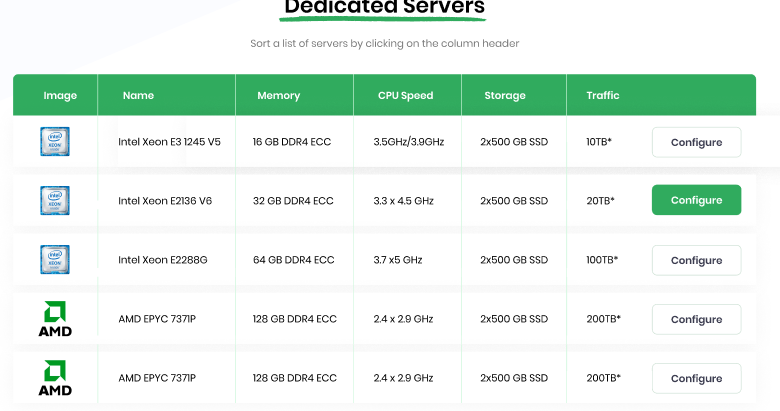
\includegraphics[width=0.9\linewidth]{7_3}
		\caption{selecting best candidate system}
		\label{fig:73}
	\end{figure}
\end{itemize}
\section{Conclusion}
In this chapter we learn about feasibility study.
A feasibility study is conducted to select the best system that meets performence requirement .Three consideration are :economic,technical and behavioral .Economic analysis as cost/benefit .techincal evaluate existing cost/benifit,and they follow the feasibility steps to build a project successfully.





\chapter{Cost/Benefit Analysis}
\section{Intoduction}
A cost-benefit analysis is the process of comparing the projected or estimated costs and benefits (or opportunities) associated with a project decision to determine whether it makes sense from a business perspective.\\
\section{Data analysis}
Data analysis is a prerequisite to cost/benefit analysis. For Netacode,a single statement that succinctly defines clint product/service\\
- Fast , Secure and Reliable
\section{cost}
Cost determine the benifit and seving that are expected from the system and compare them with the expected costs.\\
\\The cost for a project mainly depend on time,server,hardware ,equipment and personnel cost.
\subitem \textbf{Hardware/software cost:\\}It include the cost of purchasing or leasing of computers and its peripherals.Software cost involves required software cost.

\begin{figure}[h]
	\centering
	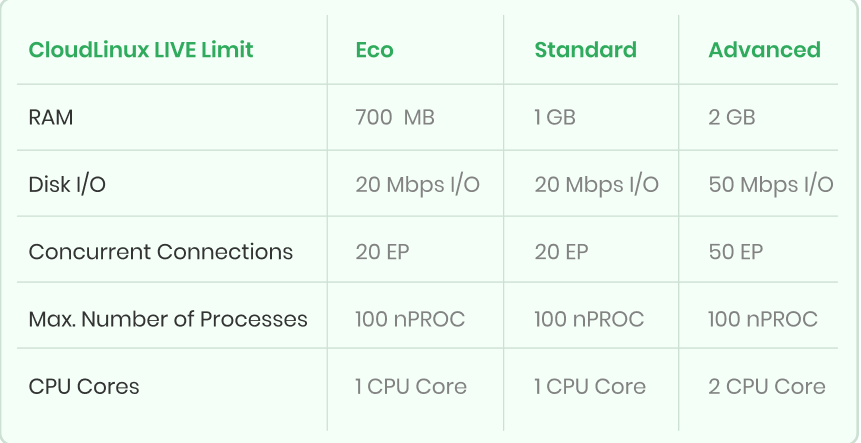
\includegraphics[width=0.7\linewidth]{7_2}
	\caption{using hardware list}
	\label{fig:72}
\end{figure}

\subitem \textbf{personnel cost:\\}It is the money send on the people involve in the development the project .These expenditures include salaries,other benifit such as health ,conveyance allowance etc.In netacode
each personnel cost is 50000 per month and forevery project extra working per hours they pay extra 5000.
\subitem \textbf{Time cost:} 
If a project need to made by personnel more time ,give them more money.\\ \\
\begin{figure}[h]
	\centering
	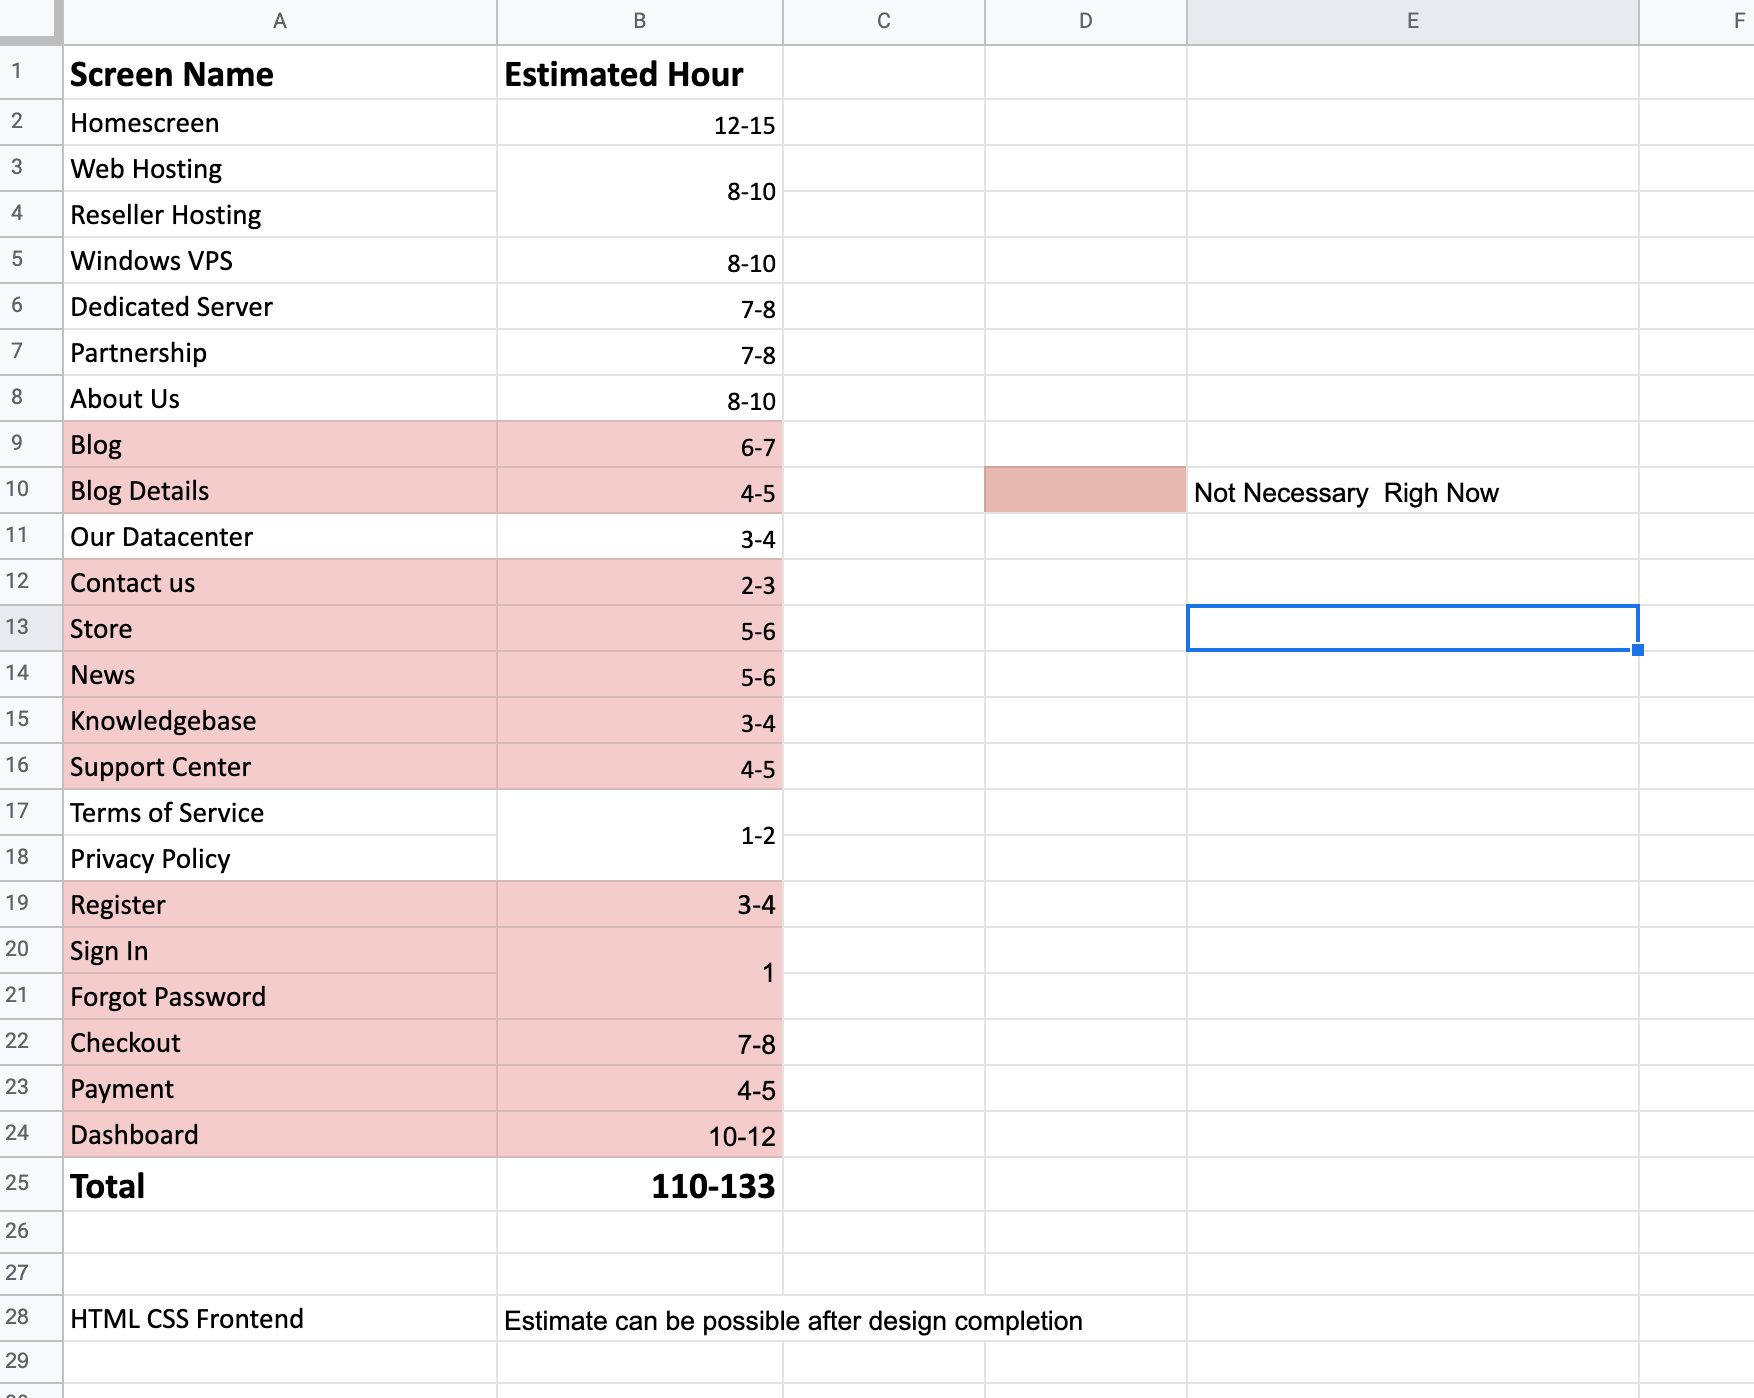
\includegraphics[width=1 \linewidth]{8_1}
	\caption{Time requirement for a website ECNHOST made by NetaCode }
	\label{fig:81}
\end{figure}
\subsection{Cost analysis for a existing project}
Successfully run a project by Netacode cost analysis\\
Total Investment by clint is 3,550,000tk
\begin{center}
	Ten member work in this project for 15 days.\\
	personnel cost =(10*50,000)+(5000*3*10)=6,50,000tk\\
	hardware/software cost=5,00000tk\\
	equipment cost=20,00000tk\\
	Others=4,00000\\
\end{center}
\begin{center}
	total=650000+500000+2000000+400000\\
	=3550000tk\\
\end{center}

\section{Benefit}
The biggest advantage of Netacode audience is that -
\begin{itemize}
	\item	clint can start with their services without any technical
	knowledge , as we will provide full support for them.
	\item Very Economical ( We can beat any of our competitors) with ensuring quality service
	\item Multi-Carrier Route Optimized Network
	\item Proactive monitoring and resolution
	\item Exceptional performance and reliability
	\item Best customer retention rate
	\item 24 hours Live Support by responsible and reliable Staff.
\end{itemize} 
\subsection{Benefit analysis for a existing project}
After running the project average every month in first One year  earn by clint 150,000.\\
so,No.of month  need for net benifit\begin{center}
	n=3,550,000/200,000=~18 month=~1.8 year \\
	and every month server cost pay  by clint is 10,000tk
	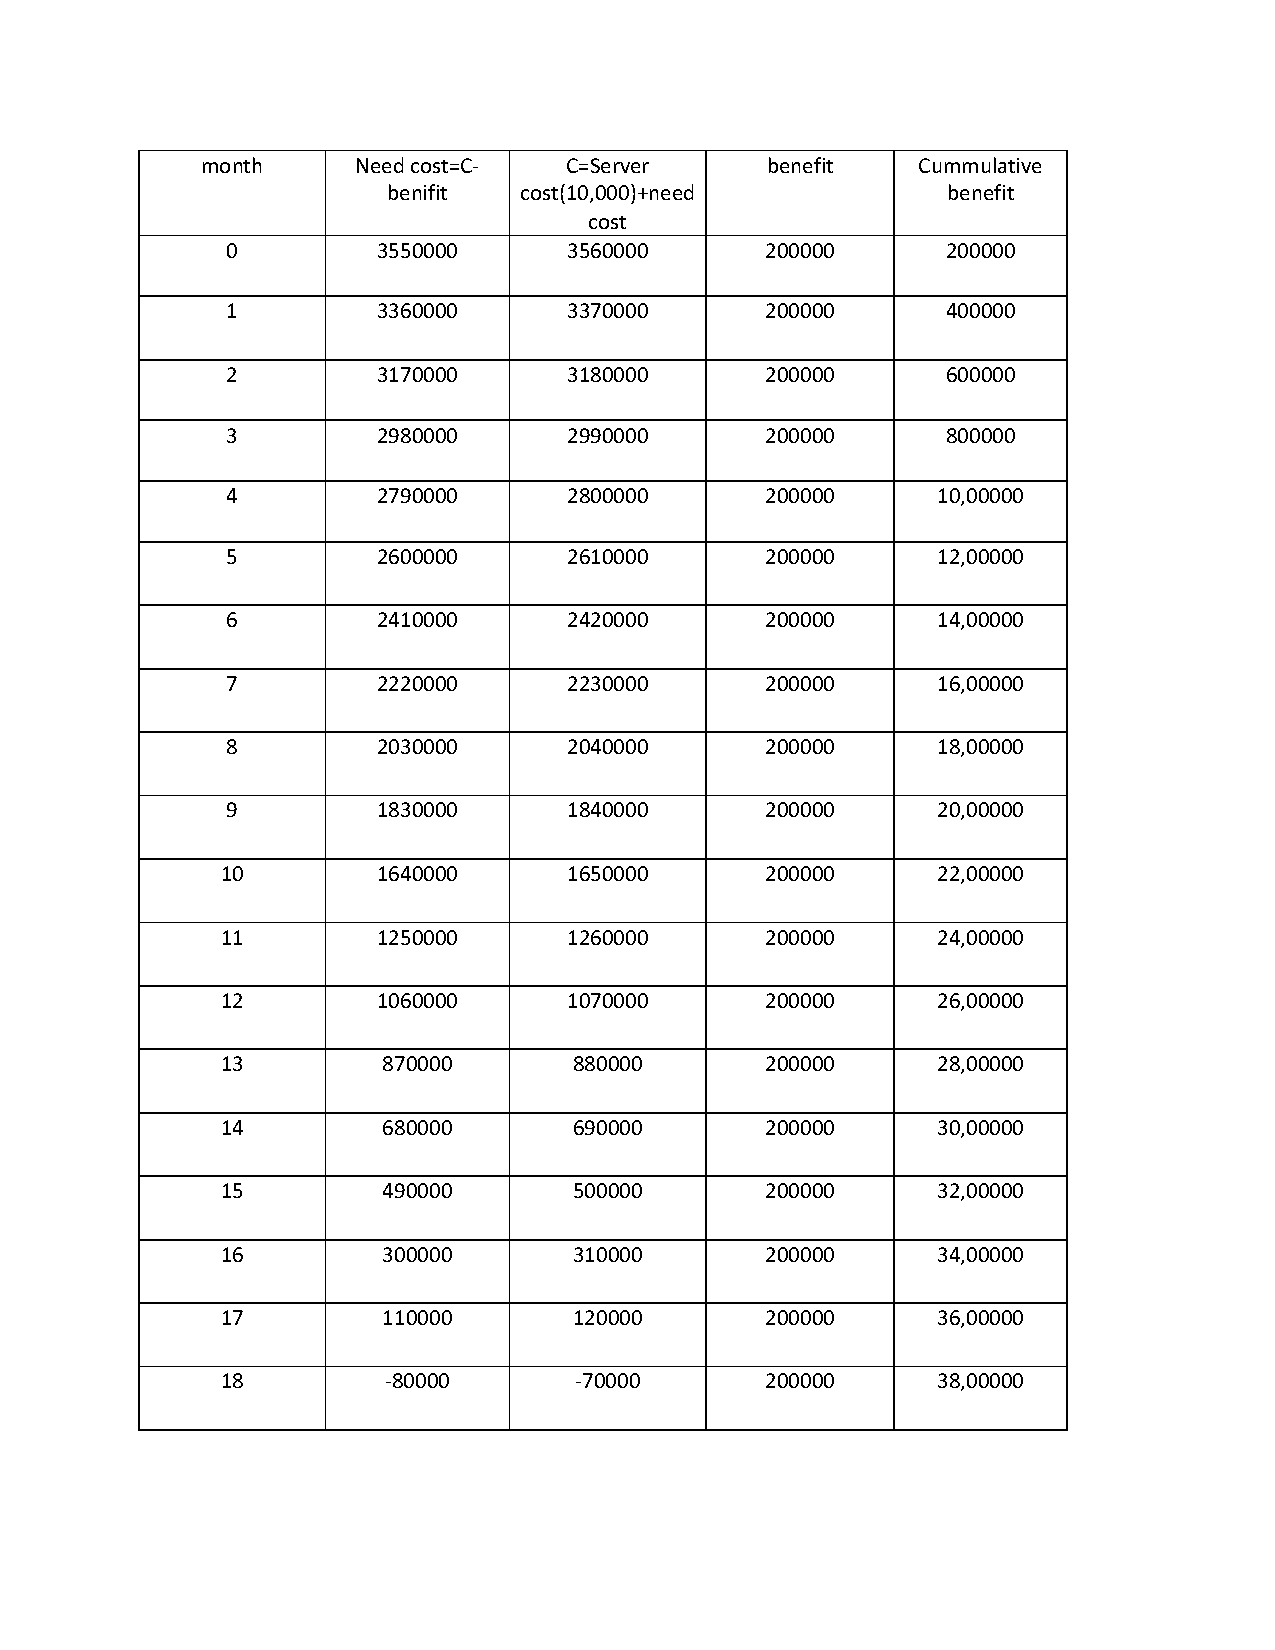
\includepdf[pages={1}] {cost.pdf}
\end{center} 
So after 18 month running this project the clint get 20,0000tk profit every month
\begin{figure}[h]
	\centering
	
\includegraphics[width=0.8\linewidth]{8_4}
	\caption{NetaCode services}
	\label{fig:84}
\end{figure}
\section{Conclusion}
Cost benefit and data analysis is most Important think for every system.we can find the existing system is benifited or not after analysis cost and benefit analysis.Clint can decide the want run the system after seeing the cost analysis.








\chapter{The Process and Stages of System Design}	
\section{Introduction}
The discussion is so far to a pivotal point in the system development life cycle. User requirements have been identified. Information has been gathered to verify the problem and evaluate the existing system. A feasibility analysis has been conducted to review alternative solutions and provide cost/benefit justification.  The culmination of the study is a proposal summarizing the finding and recommending a candidate system for the user.\\
\textbf{The design phase is a translation from a user-oriented document to a document oriented to the programs or database personnel.} 
\section{Logical and Physical Design}

System design goes through two phases of development: logical and physical design. The design which shows the logical flow of a system and defines the boundaries of the system is known as \textbf{logical system design}. It describes the input,output,databases and procedures all in a format that meets the user requirements. The design Netacode covers the following: 
\begin{enumerate}
	\item	Reviews the current physical system: its data flow , frequencies.
	\item 	Prepares output specification:it determines the format content and frequency of reports.
	\item 	Prepares input specification: format, content and most of the input functions
	\item 	Specifies the implementation plan.
	\item	Review benefits , costs, target dates and system constraints.
\end{enumerate}
\begin{figure}[h]
	\centering
	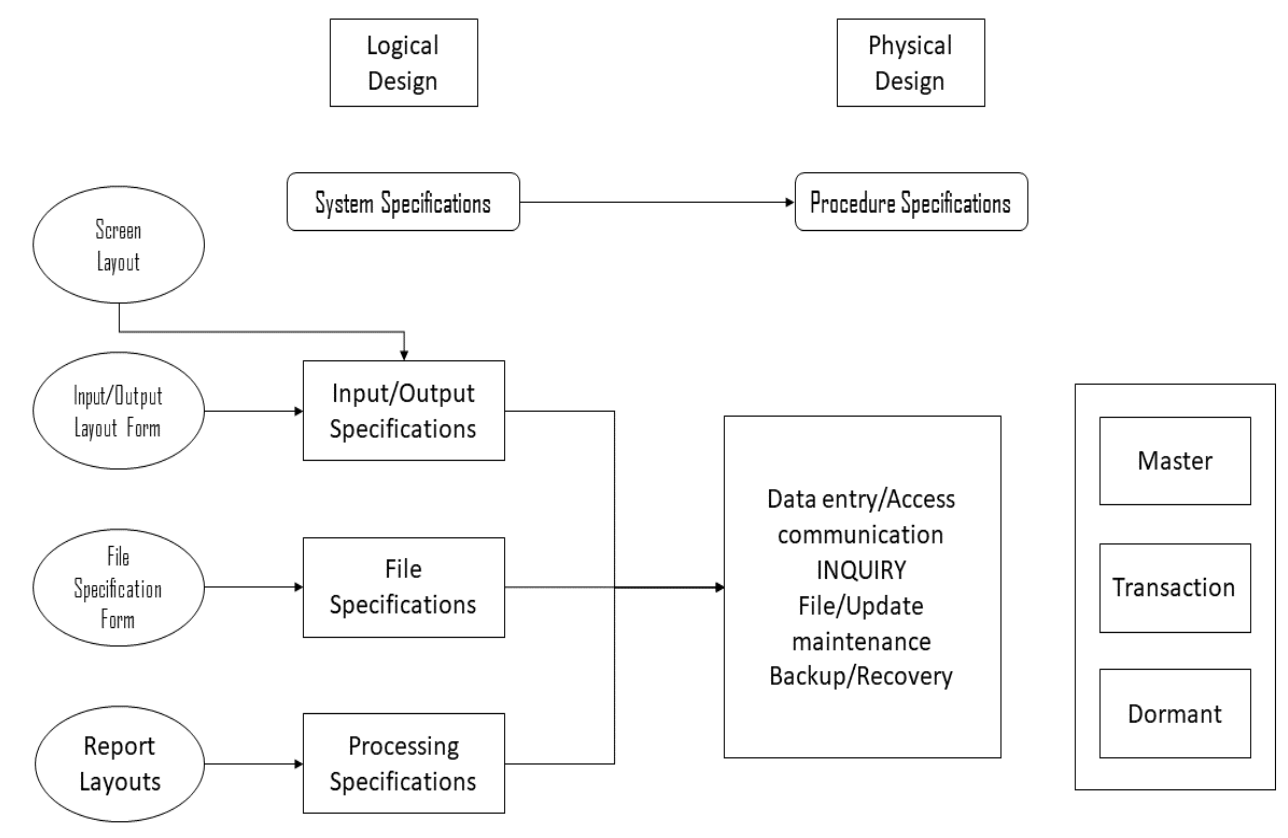
\includegraphics[width=0.9\linewidth]{9_1}
	\caption{system goes through Logical and Physical design}
	\label{fig:91}
\end{figure}
Physical design relates to the actual input and output processes of the system. It focuses on how data is entered into a system,verified, processed and displayed as output. It produces the working system by defining the design specification that specifies exactly what the candidate system does. It consist of following steps for Netacode:	

\begin{itemize}
	\item Specifying the input/output media, designing the database, and specifying    backup won server.
	\item  Planning system implementation.
	\item  Devising a test and implementation plan, and specifying any new hardware         and software.
	\item  Updating costs, benefits, conversion dates, and system constraints.
	
\end{itemize}
\section{Structured Design}

Structured design is a data-flow-based methodology.  In structured designing, the system specifications act as a basis for graphically representing the flow of data and sequence of processes involved in a software development with the help of DFDs.The figure 9.3 shows the HIPO diagram of Netacode.


\begin{figure}[h]
	\centering
	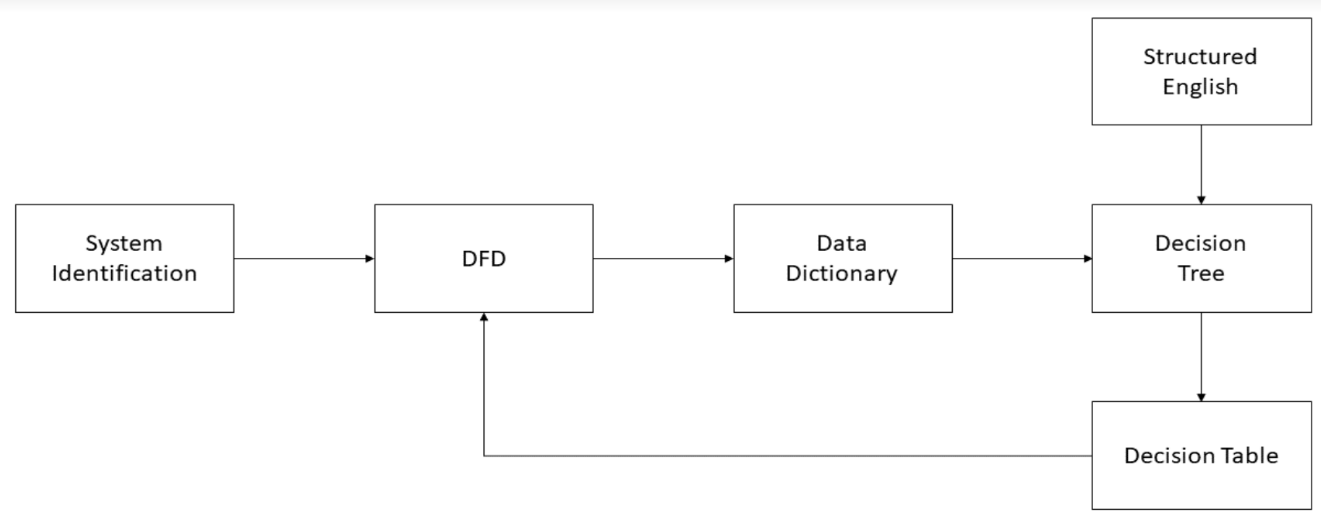
\includegraphics[width=0.8\linewidth]{9_2}
	\caption{Structured Design Method}
	\label{fig:92}
\end{figure}
\section{HIPO Diagram}
HIPO is a forms-driven technique in that standard forms are used to document the information. It consists of a hierarchy chart and an associated set of input/process/output charts. 
\begin{figure}
	\centering
	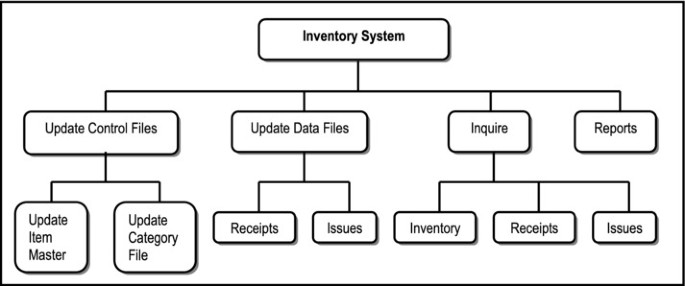
\includegraphics[width=0.7\linewidth]{9_3}
	\caption{HIPO Diagram for a project by NetaCode}
	\label{fig:93}
\end{figure}
\section{IPO Diagram}
An IPO (Input Process Output) Diagram is a very high level diagram used for system analysis that visually describes the business process with the description of each component in word. It shows a process key inputs and resulting output after a set of operations.The figure 9.4 show the IPO diagram of netacode.
\begin{figure}
	\centering
	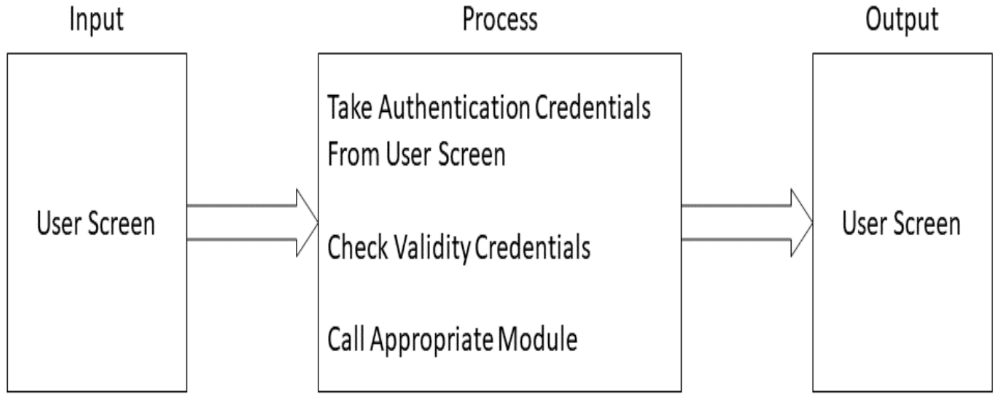
\includegraphics[width=0.7\linewidth]{9_4}
	\caption{IPO Diagram of NetaCode Implemented project}
	\label{fig:94}
\end{figure}
\section{Conclusion}
System design is the phase that bridges the gap between problem domain and the existing system in a manageable way. This focuses on the solution domain,like how to implement. It is the phase where the SRS document is converted into a format that can be implemented and decides how the system will operate. In this phase the complex activity of system development is divided into several-sub-activities. Which coordinate with each other to achieve the main objective of system development.









\chapter{Input/Output and Forms Design}
\section{Introduction}
In an information system, input is the raw data that is processed to produce output. During the input design, the developers must consider the input devices such as PC, MICR, OMR, etc.\\The design of output is the most important task of any system.
\section{Input Design}
Netacode input forms and screens have following properties 
\begin{itemize}
	\item	It should serve specific purpose effectively such as storing, recording, and retrieving the information.
	\item	It ensures proper completion with accuracy.
	\item It should be easy to fill and straightforward.
	\item	It should focus on user’s attention, consistency, and simplicity.
\end{itemize}


\section{Data Input Methods}
Some of the popular data input methods are 
\begin{itemize}
	\item 	Batch input method (Offline data input method):Clint give some ofline data to prepare a project to Netacode.
	\item 	Online data input method:sometime many online data need for develop a project.
	\item 	Computer readable forms
	\item 	Interactive data input
\end{itemize}


\section{Output Design}
Output design, developers identify the type of outputs needed, and consider the necessary output controls and prototype report layouts.

\subsection{Objectives of Output Design}
The objectives of output  design of Netacode are 
\begin{itemize}
	\item 	To develop output design that serves the intended purpose and eliminates the production of unwanted output.
	\item 	To develop the output design that meets the end users requirements.
	\item 	To deliver the appropriate quantity of output.
	\item 	To form the output in appropriate format and direct it to the right person.
\end{itemize}	
\section{Forms Design}
Both forms and reports are the product of input and output design and are business document consisting of specified data. The main difference is that forms provide fields for data input but reports are purely used for reading. For example, order forms, employment and credit application, etc.
\section{Types of Forms}
\subparagraph{Flat Forms}
\begin{itemize}
	\item	It is a single copy form prepared manually or by a machine and printed on a paper. For additional copies of the original, carbon papers are inserted between copies.
	\begin{figure}[h]
		\centering
		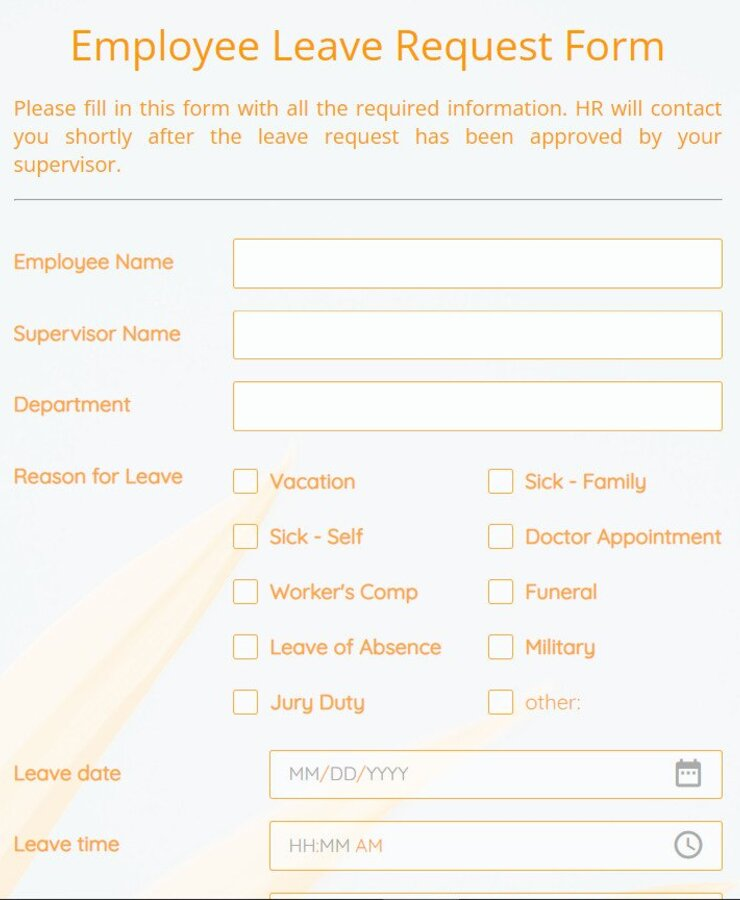
\includegraphics[width=0.6\linewidth]{employee-leave-request-form}
		\caption{Employee leave request form}
		\label{fig:employee-leave-request-form}
	\end{figure}
	\item	It is a simplest and inexpensive form to design, print, and reproduce, which uses less volume.
\end{itemize}
\subparagraph{Unit Set/Snap out Forms}
\begin{itemize}
	\item	These are papers with one-time carbons interleaved into unit sets for either handwritten or machine use.
	\item	Carbons may be either blue or black, standard grade medium intensity. Generally, blue carbons are best for handwritten forms while black carbons are best for machine use.
\end{itemize}

\section{Employment Form}
Below here is a joning leter provided by NetaCode
\begin{figure}[h]
	\centering
	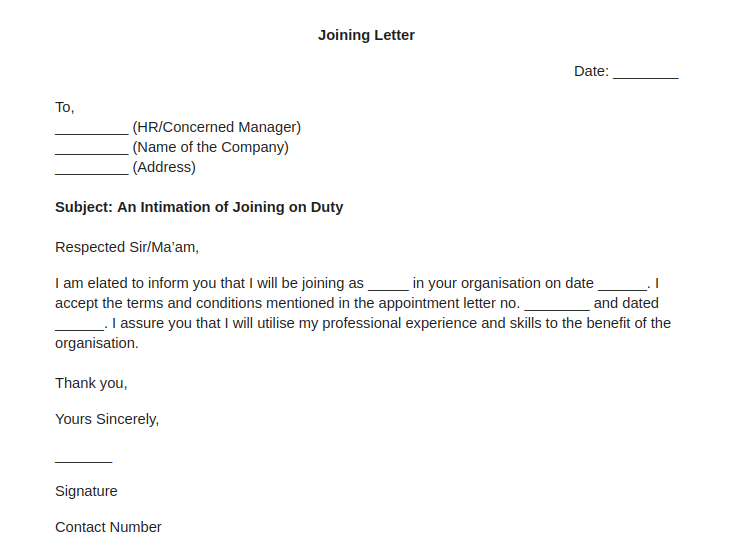
\includegraphics[width=0.8\linewidth]{10_2}
	\caption{Joning letter of Netacode }
	\label{fig:10_2}
\end{figure}

\section{Conclusion}

With their consent, the information on the form above was gathered during the visit to Netacode Inc. and used in the report. The form is used by the organization to gather project requirements from clients. This form includes Client Contact Details, Project Time frame, Project Outline, Information on existing system, Website Architecture, Design Taste, Competition and Niche, Comment Section and a Sample Project output.

\end{document}
\begin{center}
	\begin{figure}[h]
		\centering
		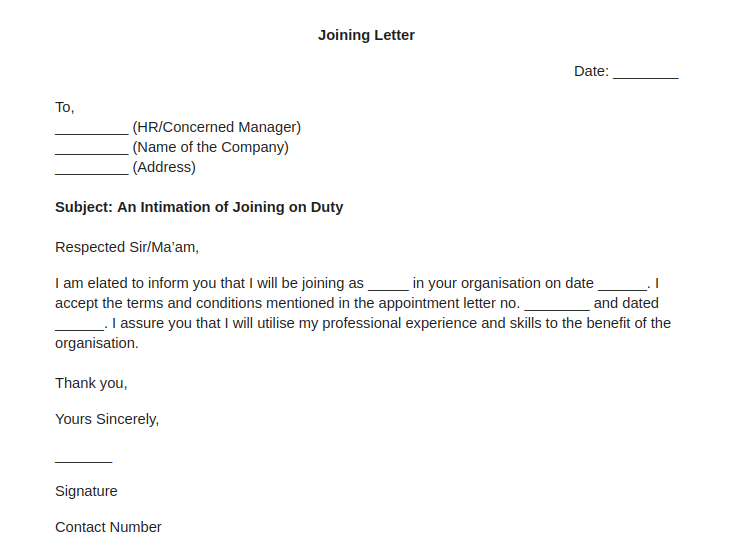
\includegraphics[width=0.8\linewidth]{10_2}
		\caption{Joning letter of Netacode }
		\label{fig:10_2}
	\end{figure}
\end{center}